% !TEX root = ../general/main.tex
\section{Application: survival after HIV}

We study the effect of a combination antiretroviral therapy versus zidovudine (ZDV) monotherapy on event-free survival in HIV.
We combine the AIDS Clinical Trials Group Protocol~175 (ACTG~175) \citep{hammer1996} with the Multicenter AIDS Cohort Study (MACS) \citep{kaslow1987}.
Treatment in ACTG~175 is randomised.
MACS is an observational cohort with unmeasured confounding \citep{hernan2000marginal}.
We pool the three combination regimens in ACTG~175 into one comparator and contrast it with ZDV monotherapy.
We restrict both sources to a common population: men with baseline CD4 count of 200 to 500 cells/mm$^3$.
This alignment makes the fusion credible, since the two sources then approximate one population \citep{pocock1976}.
We adjust for six baseline covariates: age, CD4, CD8, calendar year, race, and years of prior antiretroviral therapy.
Table~\ref{tab:cohort} summarises the aligned cohort: 1771 trial patients and 373 cohort patients.
The trial follows patients for a maximum of about three years: too short to reach median event-free survival.
The cohort follows them for about twenty-five years and reaches a median event-free survival of five to six years.
This longer follow-up adds robustness for the late treatment effect where the trial is uninformative.
MACS records outcomes at biannual visits. 
The data give event times only to the calendar year, so the events are interval-censored at annual resolution.
Figure~\ref{fig:km-curves} shows the Kaplan--Meier survival curves.

\begin{table}[b]
  \centering
  \begin{tabular}{@{}lcc@{}}
    \toprule
                                    & ACTG~175 (RCT)  & MACS (RWD)        \\
    \midrule
    Age, y                          & 34 [29, 41]     & 39 [34, 44]      \\
    CD4, cells/mm$^3$               & 337 [263, 422]  & 263 [178, 365]   \\
    CD8, cells/mm$^3$               & 918 [670, 1246] & 849 [659, 1153]  \\
    Calendar year                   & 1992            & 1991 [1991, 1992]\\
    Prior ART, y                    & 0.4 [0, 2.1]    & 1.0 [0, 1]       \\
    Non-white, $n$ (\%)             & 404 (23)        & 78 (21)          \\
    \bottomrule
  \end{tabular}
  \caption{Characteristics of the trial-aligned analysis cohort of
    $2{,}144$ patients, by data source. Continuous variables are reported
    as median [IQR], categorical variables as $n$ (\%). }
  \label{tab:cohort}
\end{table}



\begin{figure}[tb]
  \centering
  
\includegraphics[width=0.8\linewidth]{survival_curves_manuscript.pdf}
  \caption{Kaplan--Meier curves of event-free survival, by data source
    (RCT, RWD) and treatment group (ZDV monotherapy and combination).
    The main panel spans the full cohort follow-up of about 25 years;
    the inset zooms to the shorter trial window. The cohort curves are
    approximate due to interval censoring.}
  \label{fig:km-curves}
\end{figure}


We fit a Bayesian fusion forest to the combined data with default settings.
We compare it with an AFT Bayesian causal forest fitted to the trial alone.
We compute the average effect with a source-specific Bayesian bootstrap.
The source weights follow a Dirichlet prior proportional to the sample sizes.
The fusion estimate of the average acceleration factor is $1.65$ (95\% CrI: $1.43$ to $1.90$).
The trial-only baseline is close at $1.70$ (95\% CrI: $1.51$ to $1.92$).
Combination therapy stretches the event-free survival time scale by a factor of $1.65$ relative to monotherapy. 
Equivalently, the median event-free survival time under combination therapy is $1.65$ times the median under monotherapy.


The treatment effect varies across patients.
Figure~\ref{fig:cate} shows the subject-level acceleration factor for every patient, ordered by posterior mean.
The estimates lie above one, so combination helps almost everyone.
The size of the gain differs across patients.
The fusion intervals are far narrower than the trial-only intervals, which we report in the appendix.
The cohort therefore sharpens the individual estimates, not only the average.

\begin{figure}[tb]
  \centering
  
\includegraphics[width=0.8\linewidth]{cate_caterpillar_manuscript.pdf}
  \caption{Subject-level acceleration factor for every
    patient in the trial-aligned cohort, from the Bayesian fusion forest,
    ordered by posterior mean. Vertical bars are pointwise 95\%
    credible intervals; colour indicates the data source (RCT, RWD);
    the dashed line at $1$ marks no effect.}
  \label{fig:cate}
\end{figure}

We investigate how the treatment effect varies across patients. 
We use the two-stage idea behind the Virtual Twins method \citep{foster2011subgroup}.
The first stage estimates a per-patient effect, and the second fits a simple model to these estimates to locate where the effect varies.
We adapt the idea to the fusion forest as a posterior summary.
We fit the second-stage model to the posterior-mean effect and read its uncertainty from the full posterior.

We summarise the treatment effect with a regression tree (CART; \citealp{breiman1984cart}).
Figure~\ref{fig:fit-the-fit} shows a depth-three tree on the six covariates.
It splits on CD8 count and race.
The other covariates do not enter.
The acceleration factor rises with CD8, from about $1.5$ in the lowest group to about $1.8$ in the highest.
White patients gain slightly more than non-white within each CD8 band.
Every leaf exceeds $1.4$, so all subgroups benefit.
The benefit is largest at high CD8.

% Fit-the-fit summary of the FusionForest CATE.  TikZ-drawn so the
% manuscript controls the typography.  Numbers below are read off
% notes/general/figures/fit_the_fit_manuscript.pdf and matched to
% data/analysis 1/analysis_fit_the_fit.txt.
\definecolor{splitfill}{RGB}{230,244,250}
\begin{figure}[b]
  \centering
  % First arg of \resizebox is the target width -- change this fraction
  % to scale the whole figure uniformly (height auto-follows via !).
  \resizebox{0.8\textwidth}{!}{%
  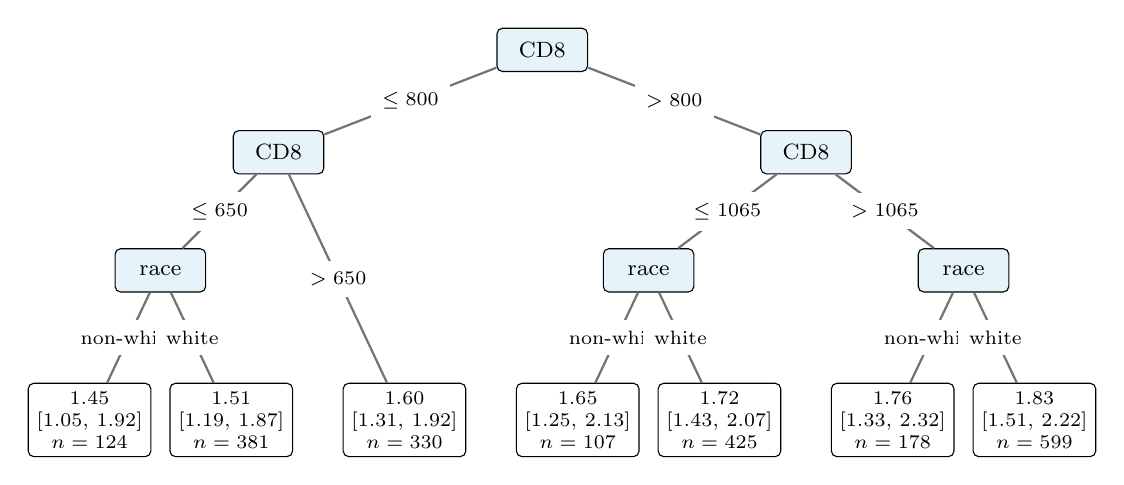
\begin{tikzpicture}[
    every node/.style = {align=center, font=\footnotesize},
    splitn/.style     = {draw, rounded corners=2pt, fill=splitfill,
                         minimum width=1.15cm, minimum height=0.55cm,
                         inner sep=2.5pt},
    leafn/.style      = {draw, rounded corners=2pt, fill=white,
                         minimum width=1.45cm, minimum height=0.85cm,
                         inner sep=3pt, font=\scriptsize},
    elabel/.style     = {midway, fill=white, inner sep=4pt,
                         font=\scriptsize},
    edgeln/.style     = {draw=black!55, thick}]

    % Internal (split) nodes
    \node[splitn] (root)  at ( 0.35, 4.7) {CD8};
    \node[splitn] (mid1)  at (-3.00, 3.4) {CD8};
    \node[splitn] (mid2)  at ( 3.70, 3.4) {CD8};
    \node[splitn] (raceA) at (-4.50, 1.9) {race};
    \node[splitn] (raceB) at ( 1.70, 1.9) {race};
    \node[splitn] (raceC) at ( 5.70, 1.9) {race};

    % Leaves
    \node[leafn] (L1) at (-5.4, 0) {$1.45$\\$[1.05,\,1.92]$\\$n = 124$};
    \node[leafn] (L2) at (-3.6, 0) {$1.51$\\$[1.19,\,1.87]$\\$n = 381$};
    \node[leafn] (L3) at (-1.4, 0) {$1.60$\\$[1.31,\,1.92]$\\$n = 330$};
    \node[leafn] (L4) at ( 0.8, 0) {$1.65$\\$[1.25,\,2.13]$\\$n = 107$};
    \node[leafn] (L5) at ( 2.6, 0) {$1.72$\\$[1.43,\,2.07]$\\$n = 425$};
    \node[leafn] (L6) at ( 4.8, 0) {$1.76$\\$[1.33,\,2.32]$\\$n = 178$};
    \node[leafn] (L7) at ( 6.6, 0) {$1.83$\\$[1.51,\,2.22]$\\$n = 599$};

    % Edges
    \draw[edgeln] (root) -- (mid1)  node[elabel] {$\le 800$};
    \draw[edgeln] (root) -- (mid2)  node[elabel] {$> 800$};

    \draw[edgeln] (mid1) -- (raceA) node[elabel] {$\le 650$};
    \draw[edgeln] (mid1) -- (L3)    node[elabel] {$> 650$};
    \draw[edgeln] (mid2) -- (raceB) node[elabel] {$\le 1065$};
    \draw[edgeln] (mid2) -- (raceC) node[elabel] {$> 1065$};

    \draw[edgeln] (raceA) -- (L1) node[elabel] {non-white};
    \draw[edgeln] (raceA) -- (L2) node[elabel] {white};
    \draw[edgeln] (raceB) -- (L4) node[elabel] {non-white};
    \draw[edgeln] (raceB) -- (L5) node[elabel] {white};
    \draw[edgeln] (raceC) -- (L6) node[elabel] {non-white};
    \draw[edgeln] (raceC) -- (L7) node[elabel] {white};
  \end{tikzpicture}}
  \caption{Regression-tree summary of the acceleration factor
    $\exp\{\tau(x)\}$ from the fusion forest. We fit the tree to the
    posterior-mean log-time CATE on the six baseline covariates. Each leaf
    gives the within-leaf average acceleration factor, as a posterior mean
    and 95\% credible interval.}
  \label{fig:fit-the-fit}
\end{figure}

We inspect the posterior probability of treatment benefit $ \p(\tau(x_i) > 0 \mid \text{data})$ for each patient \citep{henderson2020individualized}.
We bin the patients by posterior probability of benefit and report the fraction in each bin.
We compute it over the trial population, under the fusion and trial-only fits, so the columns are comparable (Table~\ref{tab:hte-summary}).
We find strong evidence of benefit for almost every patient: $77\%$ have $\pi_i > 0.99$ and $97\%$ exceed $0.95$.
The trial alone is far less certain, with only $38\%$ above $0.95$ and a quarter of patients inconclusive.
The Bayesian fusion forest gains this certainty even though its average effect is slightly smaller ($1.65$ versus $1.70$).

We also summarise the between-source heterogeneity in baseline prognosis.
We fit a best-linear projection to the deviation forest  \citep{Woody2020}.
The deviation forest $d(x)$ measures how the baseline prognosis differs between the trial and the cohort.
We project $d(\cdot)$ onto the covariates by least squares.
We present the results in Table~\ref{tab:projection}.
The gap is dominated by a constant shift.
The intercept is $1.70$ (95\% CrI: $1.31$ to $2.10$), so the cohort baseline sits well above the trial.
Among the covariates, only prior antiretroviral years moves the gap, by $0.27$ (95\% CrI: $-0.01$ to $0.55$).
Age, CD4, CD8, calendar year, and race have coefficients near zero, with intervals covering zero.
The baseline prognosis therefore differs mainly through a large average shift.
This shift likely reflects population and measurement differences the six covariates do not capture.


Combination therapy prolongs event-free survival by a factor of about $1.65$.
The cohort's Kaplan--Meier curves do not reveal this benefit.
The Bayesian fusion forest recovers the effect.
The combined analysis also sharpens the individual estimates.
We identify benefit for nearly every patient, far more than the trial alone.
The treatment effect varies with CD8 count and race.
The baseline prognosis differs between the sources, through a gradient in prior antiretroviral exposure and a large average shift.

\begin{table}[tb]
  \centering
  \begin{minipage}[t]{0.46\textwidth}
    \centering
    \small
    \begin{tabular}{@{}lcc@{}}
      \toprule
      $\p(\tau(x_i) > 0 \mid \text{data})$        & Fusion & Trial-only \\
      \midrule
      $(0.99, 1]$    & $0.767$ & $0.180$ \\
      $(0.95, 0.99]$ & $0.206$ & $0.198$ \\
      $(0.75, 0.95]$ & $0.028$ & $0.364$ \\
      $(0.25, 0.75]$ & $0.000$ & $0.245$ \\
      $[0, 0.25]$    & $0.000$ & $0.014$ \\
      \bottomrule
    \end{tabular}
    \captionof{table}{Posterior probability of benefit over the trial
      population. Higher bins give stronger evidence of benefit, the
      lowest evidence of harm. Entries are fractions of patients.}
    \label{tab:hte-summary}
  \end{minipage}
  \hfill
  \begin{minipage}[t]{0.50\textwidth}
    \centering
    \small
    \begin{tabular}{@{}lcc@{}}
      \toprule
      Term          & Coefficient & 95\% CrI \\
      \midrule
      Intercept     & $1.701$  & $(1.312, 2.099)$ \\
      \midrule
      Age           & $-0.003$ & $(-0.020, 0.015)$ \\
      CD4           & $0.001$  & $(-0.001, 0.002)$ \\
      CD8           & $0.000$  & $(-0.000, 0.000)$ \\
      Calendar year & $-0.032$ & $(-0.256, 0.194)$ \\
      Race          & $0.071$  & $(-0.304, 0.443)$ \\
      Prior ART, y  & $0.269$  & $(-0.008, 0.550)$ \\
      \bottomrule
    \end{tabular}
    \captionof{table}{Best linear projection of the deviation forest
      $d(x)$ onto the covariates: posterior mean coefficient and 95\%
      credible interval on the log-transformed time scale.}
    \label{tab:projection}
  \end{minipage}
\end{table}
